\UseRawInputEncoding
\documentclass[12pt]{article}
\usepackage[utf8]{inputenc}
\usepackage{graphicx}
\usepackage[table]{xcolor}
\usepackage{hyperref}
\usepackage{tikz}
\usepackage{amsmath}
\usepackage{pgf, tikz} % Graphs
\usetikzlibrary{arrows, automata} % Graphs
\usetikzlibrary{shapes,trees,positioning}
\hypersetup{
    colorlinks=true,
    linkcolor=blue,
    filecolor=magenta,
    urlcolor=tumgadBlue,
}
\usepackage[a4paper, total={6in, 9in}]{geometry}
\usepackage[nodisplayskipstretch]{setspace}
\usepackage[printwatermark]{xwatermark}
\usepackage{enumitem,amssymb}
\definecolor{tumgadPurple}{RGB}{105,0,168}
\definecolor{tumgadBlue}{RGB}{79, 100, 255}
\definecolor{tumgadRed}{RGB}{255,85,85}
\newcolumntype{P}[1]{>{\centering\arraybackslash}p{#1}} % Center column values in content table

% Header/Footer definitions
\lhead{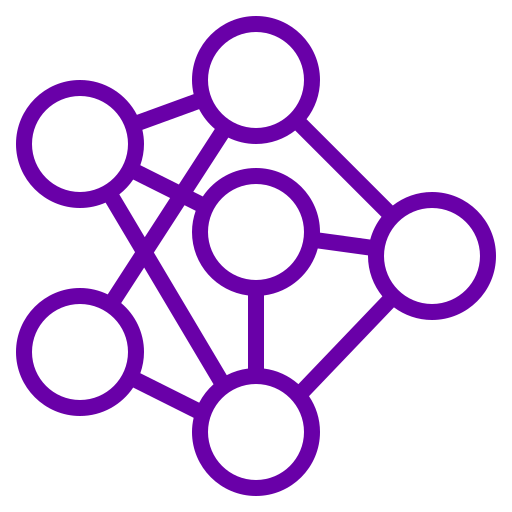
\includegraphics[scale=0.03]{favicon.png} TUMGAD - Exercises}
\rhead{\thepage}
\renewcommand{\headrulewidth}{0.4pt}
\usepackage{fancyhdr}
\pagestyle{fancy}
\cfoot{TUMGAD was created by Sebastian Oßner and Daniel Krüger \href{https://github.com/SebastianOner/TUMGAD}{\underline{View it on GitHub}}}
\renewcommand{\footrulewidth}{0.4pt}

\begin{document}

    \begin{center}
        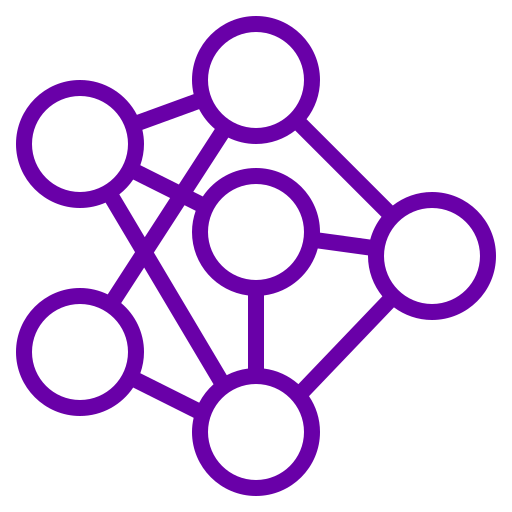
\includegraphics[scale=0.25]{favicon.png} % favicon made by Becris on https://flaticon.com
        \vspace{15px}

        {\fontfamily{Inconsolata}\selectfont
            \textbf{\LARGE{TUMGAD - Exercises}}\\
            Generated: $GENERATEDDATE$\\
            Seed: $RANDOMSEED$\\
        }
        \vspace{20px}
        \textbf{\LARGE{-----Disclaimers and Infos:-----}}
        \\[0.2in]
    \end{center}
    1. You can find explanations to all the components in this repository and instructions on how to use the generator \href{https://sebastianoner.github.io/TUMGAD/src/routes}{\underline{here}}.
    \\[0.2in]
    2. This paper was generated by an automated software.
    It might contain flaws.
    If you find one (or even think you've found one), please report it \href{https://github.com/SebastianOner/TUMGAD/issues/new?assignees=&labels=&template=bug_report.md&title=}{\underline{here}}.
    \\[0.2in]
    3. TUMGADs creators are not affiliated with the lecture organization whatsoever, the exercises/explanations are not
    guaranteed to be accurate or complete.
    \\[0.2in]
    4. The algorithms in this tool are sometimes substantially oversimplified, this is due to the students having to execute them by hand in exams
    and thus it is impractical to increase the difficulty (e.g. RadixSort only deals with 3-digit numbers).
    \\[0.2in]
    5. If you like this tool, a good thing you can do is spread the word or star the \href{https://github.com/SebastianOner/TUMGAD/}{\underline{repo on GitHub}} to help out more of your fellow students as well as the creators.
    \vspace{20px}
    \begin{center}
        % Table containing information about the exercises in this paper. in an included exercise the
        % placeholders are replaced with \cellcolor{tumgadPurple}, if it's excluded, the cell is white
        % If compiled without placeholders, it will look terrible, as equations don't break the line at cell-end
        \begin{tabular}{|P{4cm}|P{1cm}||P{4cm}|P{1cm}|}
            \hline
            Arrays & %$ARRAYS$
            & Hashing w/ Chaining & %$HashingChaining$
            \\ \hline
            Double Hashing & %$DoubleHashing$
            & MergeSort & %$MergeSort$
            \\ \hline
            QuickSort & %$QuickSort$
            & RadixSort & %$RadixSort$
            \\ \hline
            Binary Heaps & %$BINARYHEAPCELL$
            & BinomialHeaps & %$BINOMIALHEAPCELL$
            \\ \hline
            AVL Trees & %$AVLCELL$
            & AB Trees & %$ABCELL$
            \\ \hline
            BFS \& DFS & %$TRAV$
            & Dijkstra & %$DIJKSTRACELL$
            \\ \hline
            Prim & %$PRIMCELL$
            & Floyd Warshall & %$APSPFWCELL$
            \\ \hline
        \end{tabular}
    \end{center}
    %$DYNAMICARRAYS$
    %$HASHINGCHAINING$
    %$DOUBLEHASHING$
    %$MERGESORT$
    %$QUICKSORT$
    %$RADIXSORT$
    %$BINARYHEAPS$
    %$BINOMIALHEAPS$
    %$AVLTREES$
    %$ABTREES$
    %$TRAVERSAL$
    %$DIJKSTRA$
    %$PRIMALGORITHM$
    %$FLOYDWARSHALL$
\end{document}